\chapter{Convolutional Neural Networks}
\section{Motivation}
There exist a complex arrangement of cells within the visual cortex. These
cells are sensitive to small sub-regions of the input space, called a
\textbf{receptive field}, and are tiled in such a way as to cover the
entire visual field. These filters are local in input space and are thus
better suited to exploit the strong spatially local correlation present in
natural images.

Two basic cell types: Simple cells (S) and complex cells (C).
\begin{itemize}
    \item Simple Cells(S) respond maximally to specific edge-like stimulus
        patterns within their receptive field.
    \item Complex cells(C) have larger receptive fields and are locally
        invariant to the exact position of stimulus.
\end{itemize}

\section{Sparse Connectivity}
CNNs exploit spatially local correlation by \textbf{enforcing a local
connectivity pattern between neurons of adjacent layers}. 

Input hidden units in the $m$-th layer are connected to a local subset of
units in the $(m-1)$-th layer, which have spatially contiguous receptive
fields. 

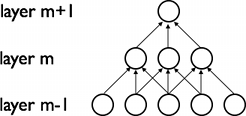
\includegraphics{sparse_1D_cnn}

\begin{itemize}
    \item Layer $m-1$ is the input retina. 
    \item Units in layer $m$ have receptive fields of width 3. Thus only
        connected to 3 adjacent neurons in the $(m-1)$-th layer.
    \item Layer $m$ have a similar connectivity with the layer below.
        $(m+1)$
\end{itemize}

We say that their receptive field with respect tot he layer below is 3,
but their receptive field with respect to the input is larger (it is 5).
The architecture thus confines the learnt ``filters'' to the spatially
local pattern.

\section{Shared Weights}
In CNNs, each sparse filter $h_i$ is additionally replicated across the
entire visual field. These ``replicated'' units form a \textbf{feature
map}, which share the same parameterization. (the receptive fields in the
same feature map share the same weight and bias for the sensitive region)

Gradient descent can still be used to learn such shared parameters, and
requires only a small change to the original algorithm. The gradient of a
shared weight is simply the sum of the gradients of the parameters being
shared.

Replicating units in this way allows for feature to be detected regardless
of their position in the visual field. Additionally, weight sharing offers
a very efficient way to do this, since it greatly reduces the number of
free parameter 

\section{Details and notation}
The $k$-th feature map at a given layer as $h^k$, whose filter with
weights $W^k$ and bias $b_k$, then the feature map $h^k$ is obtained as
follows (for $tanh$ non-linearities)
\[ h^k_{ij} = tanh\left( \left( W^k*x)_{ij} \right) + b_k \right)\]

To form a richer representation of the data, hidden layers are composed of
a set of multiple feature maps $\left\{ h^{(k)}, k = 0\dots K \right\}$

The weights of this layer can be parameterized as a 4D tensor (Tensors are
geometric objects that describe linear relations between vectors, scalars,
and other tensors. Elementary examples of such relations include the dot
product, the cross product and linear maps, vectors and scalars themselves
are also tensors.)
\begin{itemize}
    \item Destination feature map index
    \item Source feature map index
    \item Source vertical position index
    \item Source horizontal position index
\end{itemize}
\section{MaxPooling}
MaxPooling is a form of non-linear down-sampling. MaxPooling partitions
the input image into a set of non-overlapping rectangles and, for each
such sub-region, outputs the maximum value.

Useful for two reasons:
\begin{itemize}
    \item Reduces the computational complexity for upper layers
    \item Provides a form of translation invariance
\end{itemize}

Why it works: Imagine cascading a max-pooling layer with a convolutional
layer. There are $8$ directions in which one can translate the input image
into a single pixel. If max-pooling is done over a $2\times 2$ region, 
$3$ out of these $8$ possible configurations will produce exactly the same
output at the convolutional layer. For max-pooling over a $3\times 3$

\section{The Full Model: LeNet}
Graphical depiction: 

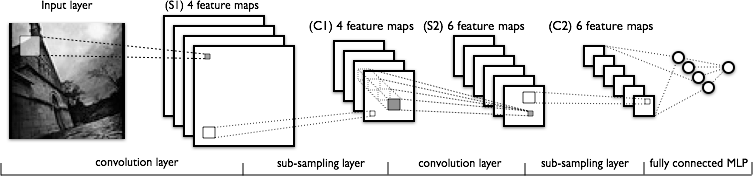
\includegraphics{mylenet}

The lower layers are composed to alternating convolution and max-mpooling
layers.

The upper layers however are fully-connected and correspond to a
traditional MLP

